\section{Test setups}\label{sec:setups}
\sectionstate{ready}{\texttt{mx\_june\_cosmic\_qa/MICROTPC\_RUNBOOK.md}; \texttt{sps\_beam\_test\_26/analysis/README.md}; \texttt{mpgd26} renders}
\intent{The two setups and what each can measure: the Saclay cosmic bench (M3 reference tracking, all five chambers,
June 2026) and the SPS H4 beam (uRWELL telescope, det4 only, including the 25.6\textdegree{} rotation).}

\subsection{Cosmic bench}
\tbw{Scintillator trigger, four M3 reference planes, two test slots. M3 recipe ($\chi^2<1.0$, $N_\mathrm{clus}=4$).
DREAM readout, sampling, window. Gas and flow.}
\askDylan{Gas per setup: bench Ar/iC$_4$H$_{10}$ 95/5? SPS runs with Ar/CF$_4$/iC$_4$H$_{10}$ 88/10/2? Which runs enter the paper?}

\begin{figure}[t]
  \centering
  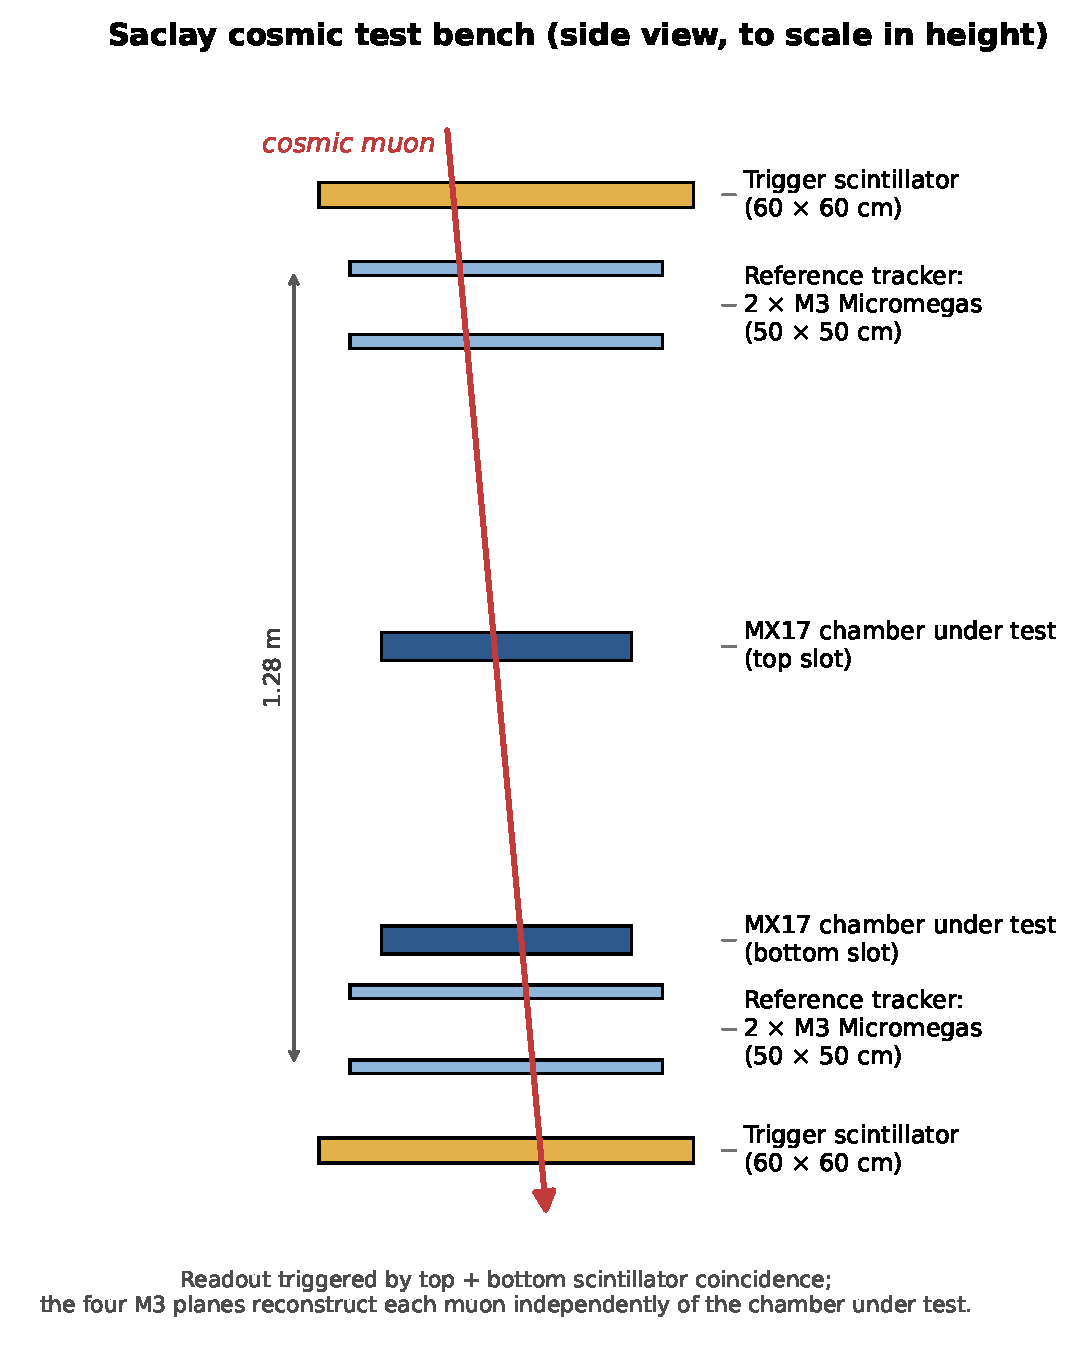
\includegraphics[width=0.75\linewidth]{bench_setup}
  \caption{The cosmic bench: scintillator trigger and four M3 reference planes around the two MX17 test slots.}
  \label{fig:bench}
\end{figure}

\subsection{SPS H4 beam}
\tbw{Beam, uRWELL references, det4 position, runs used (HV, drift field, gas, rotation).}
\begin{figure}[t]
  \centering
  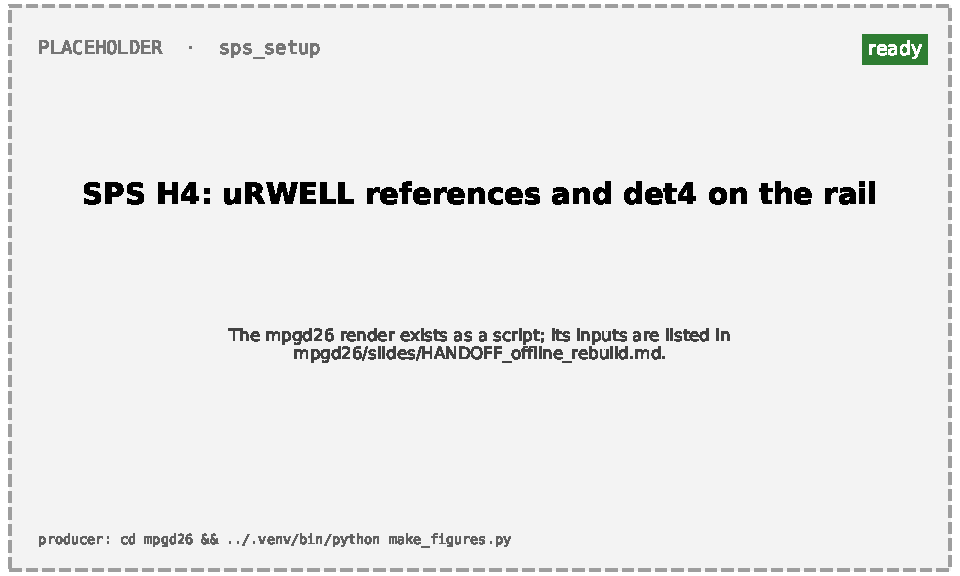
\includegraphics[width=0.85\linewidth]{sps_setup}
  \caption{\tbw{The SPS H4 setup.}}
  \label{fig:sps}
\end{figure}
